% Slide thuyet trinh (Beamer, XeLaTeX):  xelatex slide.tex (2 lan)  hoac  make slide
% Ban 10 PHUT cho ca nhom: Doanh 1' -> V.V. Duong 2.5' -> N.T. Duong 2.5' -> Dat 2.5' -> Doanh 1.5'
% Ten nguoi noi hien o chan moi slide: dat bang \nguoinoi{...} truoc cac frame.
\documentclass[aspectratio=169,11pt]{beamer}
\usepackage{fontspec}
\usepackage{amsmath}
\setsansfont{Arial}
\setmonofont{Consolas}[Scale=0.9]
\usepackage{graphicx,booktabs,tikz}
\usetikzlibrary{arrows.meta,positioning}
\graphicspath{{../../results/}}

% ---------- Giao dien ----------
\definecolor{chinh}{RGB}{20,60,120}
\definecolor{nhan}{RGB}{200,90,20}
\usetheme{default}
\setbeamercolor{frametitle}{fg=white,bg=chinh}
\setbeamercolor{title}{fg=chinh}
\setbeamercolor{structure}{fg=chinh}
\setbeamercolor{alerted text}{fg=nhan}
\setbeamerfont{frametitle}{size=\large,series=\bfseries}
\setbeamertemplate{frametitle}{\nointerlineskip\begin{beamercolorbox}[wd=\paperwidth,ht=2.4ex,dp=1.1ex,leftskip=0.5cm]{frametitle}\insertframetitle\end{beamercolorbox}}
\setbeamertemplate{navigation symbols}{}
\setbeamertemplate{itemize items}[circle]
\newcommand{\nguoi}{}
\newcommand{\nguoinoi}[1]{\renewcommand{\nguoi}{#1}}
\setbeamertemplate{footline}{\hspace{0.4cm}\color{gray}\footnotesize\nguoi\hfill\insertsection\hspace{1em}\insertframenumber/\inserttotalframenumber\hspace{0.4cm}\vspace{0.2cm}}
\newcommand{\so}[2]{\begin{minipage}[t]{3.6cm}\centering{\Huge\bfseries\color{nhan}#1}\\[2pt]\small #2\end{minipage}}
\newcommand{\code}[1]{\texttt{#1}}

\title{Song song hóa mô phỏng N-body\\bằng OpenMP và CUDA}
\author{Nguyễn Quốc Doanh (nhóm trưởng) \and Vũ Văn Dương \and Nguyễn Tùng Dương \and Trần Tiến Đạt}
\institute{Trường Đại học Khoa học Tự nhiên -- ĐHQG Hà Nội\\Học phần: Tính toán song song (MAT3148 1) -- Lớp K69A5}
\date{Tháng 11 năm 2026}

\begin{document}

\begin{frame}[plain]
\titlepage
\end{frame}

% =====================================================================
\section{Mở đầu}
\nguoinoi{Trình bày: Nguyễn Quốc Doanh}

\begin{frame}{Đặt vấn đề và mục tiêu}
\begin{columns}[T]
\begin{column}{0.5\textwidth}
\begin{itemize}
\setlength{\itemsep}{6pt}
\item $N$ vật thể hút nhau $\Rightarrow$ \alert{$N^2$ tương tác} mỗi bước
\item $N=10^5$: $2\cdot10^{11}$ FLOP/bước; một lõi CPU ($\approx$34 GFLOP/s) chạy $10^4$ bước mất $\approx$\alert{16 giờ}
\item Các tương tác trong một bước \alert{độc lập} $\Rightarrow$ bài toán mẫu để song song hóa
\end{itemize}
\end{column}
\begin{column}{0.47\textwidth}
\textbf{Bốn phiên bản, cùng đầu vào}\\[4pt]
\small
\setlength{\tabcolsep}{4pt}
\begin{tabular}{ll}
\toprule
Tuần tự & mốc so sánh, kiểm chứng \\
OpenMP & chia vòng ngoài + SIMD \\
CUDA naive & 1 luồng = 1 vật thể \\
CUDA tiled & shared memory [1] \\
\bottomrule
\end{tabular}\\[8pt]
Kiểm tra đúng $\to$ đo thời gian, speedup, hiệu suất
\end{column}
\end{columns}
\end{frame}

% =====================================================================
\section{Bài toán và lý thuyết}
\nguoinoi{Trình bày: Vũ Văn Dương}

\begin{frame}{Bài toán N-body và thuật toán tuần tự}
\begin{columns}[T]
\begin{column}{0.55\textwidth}
\[ \mathbf{a}_i = \sum_j m_j \frac{\mathbf{r}_j-\mathbf{r}_i}{\left(\lVert\mathbf{r}_j-\mathbf{r}_i\rVert^2+\varepsilon^2\right)^{3/2}} \]
\begin{itemize}
\setlength{\itemsep}{5pt}
\item \alert{Softening} $\varepsilon$: lực hữu hạn; $j=i$ tự bằng 0 $\Rightarrow$ không cần \code{if}
\item Euler đối xứng: $\mathbf{v}\mathrel{+}=\mathbf{a}\Delta t$ rồi $\mathbf{r}\mathrel{+}=\mathbf{v}\Delta t$
\item Đầu vào: cụm sao Plummer, seed 42
\end{itemize}
\end{column}
\begin{column}{0.42\textwidth}
\textbf{Mỗi bước có 2 pha}\\[6pt]
\begin{tabular}{lr}
\toprule
1. Tính gia tốc & \alert{$O(N^2)$} \\
2. Cập nhật $\mathbf{v}$, $\mathbf{r}$ & $O(N)$ \\
\bottomrule
\end{tabular}\\[8pt]
\small Pha 1 chiếm gần như toàn bộ thời gian $\Rightarrow$ cần song song hóa pha 1
\end{column}
\end{columns}
\end{frame}

\begin{frame}{Khả năng song song và độ đo hiệu năng}
\begin{columns}[T]
\begin{column}{0.52\textwidth}
\begin{itemize}
\setlength{\itemsep}{6pt}
\item Mỗi $\mathbf{a}_i$ chỉ \emph{đọc} \code{pos[]}, chỉ \emph{ghi} \code{acc[i]} $\Rightarrow$ các $i$ \alert{độc lập}, không xung đột ghi
\item $N$ việc bằng nhau $\Rightarrow$ dễ cân bằng tải
\item Giữa 2 pha cần barrier; các bước thời gian phải chạy lần lượt
\end{itemize}
\end{column}
\begin{column}{0.45\textwidth}
\[ S_p=\frac{T_1}{T_p},\qquad E_p=\frac{S_p}{p} \]
\begin{itemize}\small
\setlength{\itemsep}{4pt}
\item \textbf{Amdahl}: bài toán cố định, $S\le 1/(1-P)$
\item \textbf{Gustafson}: bài toán lớn dần; phần $O(N)$ co lại so với $O(N^2)$ $\Rightarrow$ \alert{$N$ càng lớn, speedup càng cao}
\end{itemize}
\end{column}
\end{columns}
\end{frame}

\begin{frame}{Kiểm chứng tính đúng đắn}
\begin{columns}[T]
\begin{column}{0.46\textwidth}
\begin{itemize}
\setlength{\itemsep}{6pt}
\item \code{-verify}: OpenMP khớp tuần tự \alert{từng bit}; CUDA sai khác $\approx10^{-8}$ (làm tròn \code{float})
\item $N=2048$, 2000 bước: $\Delta t>0.002$ $\Rightarrow$ sai số năng lượng tăng nhanh
\item Chọn $\Delta t=0.002$, $\varepsilon=0.01$: $|\Delta E/E_0|\approx2.7\cdot10^{-6}$
\end{itemize}
\end{column}
\begin{column}{0.52\textwidth}
\centering
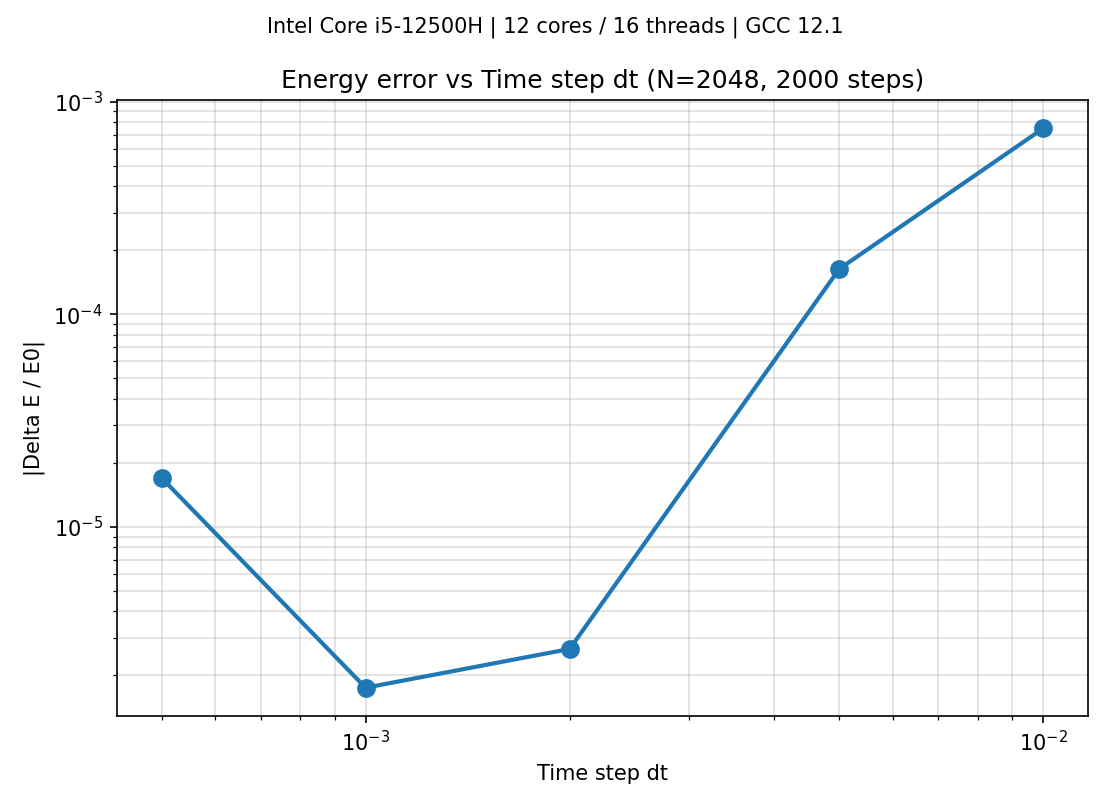
\includegraphics[width=\linewidth]{vvduong_energy_dt}
\end{column}
\end{columns}
\end{frame}

% =====================================================================
\section{OpenMP}
\nguoinoi{Trình bày: Nguyễn Tùng Dương}

\begin{frame}[fragile]{OpenMP: cách song song hóa}
\begin{columns}[T]
\begin{column}{0.54\textwidth}
\footnotesize
\begin{verbatim}
#pragma omp parallel for schedule(static)
for (i = 0; i < n; i++) {        // chia i
  #pragma omp simd reduction(+:ax,ay,az)
  for (j = 0; j < n; j++) {      // AVX2
    ... ax += dx*s; ...
  }
  acc[i] = (ax, ay, az);         // ghi riêng
}
\end{verbatim}
\end{column}
\begin{column}{0.44\textwidth}
\begin{itemize}
\setlength{\itemsep}{6pt}
\item \textbf{Fork--join}: luồng chủ tách nhóm luồng, barrier ngầm cuối vùng [2]
\item Song song 2 mức: \alert{đa luồng} (vòng $i$) + \alert{SIMD} 8 \code{float}/lệnh (vòng $j$)
\item Không cần \code{critical}/\code{atomic}
\end{itemize}
\end{column}
\end{columns}
\end{frame}

\begin{frame}{OpenMP: speedup theo số luồng (i7-13620H, 6P + 4E)}
\begin{columns}[T]
\begin{column}{0.58\textwidth}
\centering
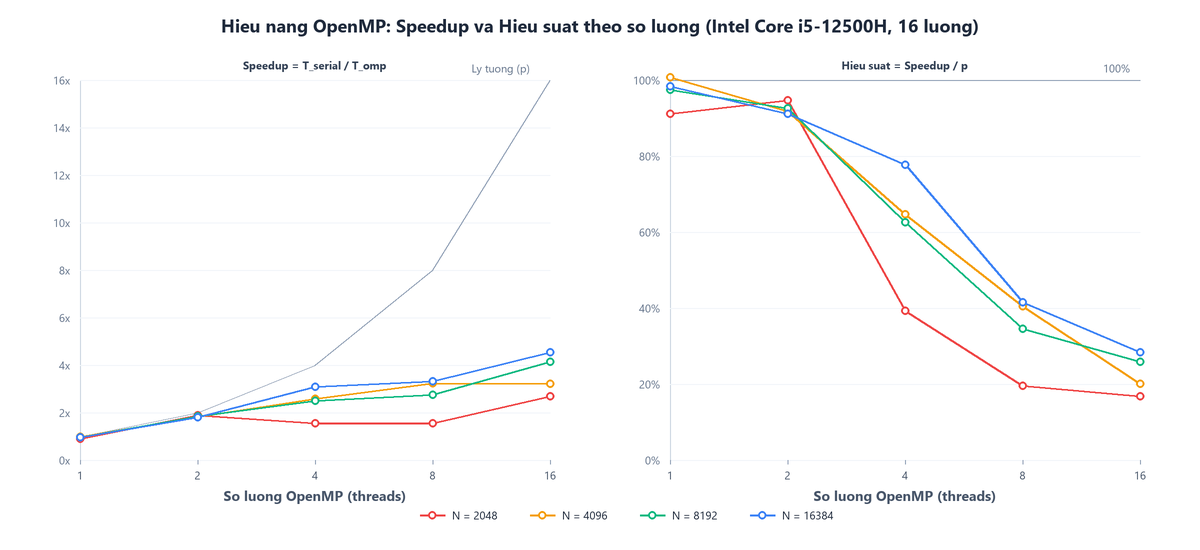
\includegraphics[width=\linewidth]{ntduong_threads_speedup}
\end{column}
\begin{column}{0.4\textwidth}
\centering
\so{5.9×}{tối đa, 16 luồng, $N=8192$ (201 GFLOP/s)}
\vspace{8pt}
\begin{itemize}\small
\item 1--4 luồng: gần tuyến tính
\item 8--16 luồng: lõi E chậm, 2 luồng chung 1 lõi P, xung nhịp giảm
\item Giới hạn do phần cứng, không phải phần tuần tự
\end{itemize}
\end{column}
\end{columns}
\end{frame}

\begin{frame}{OpenMP: SIMD, lập lịch và định luật 3 Newton}
\begin{columns}[T]
\begin{column}{0.55\textwidth}
\centering
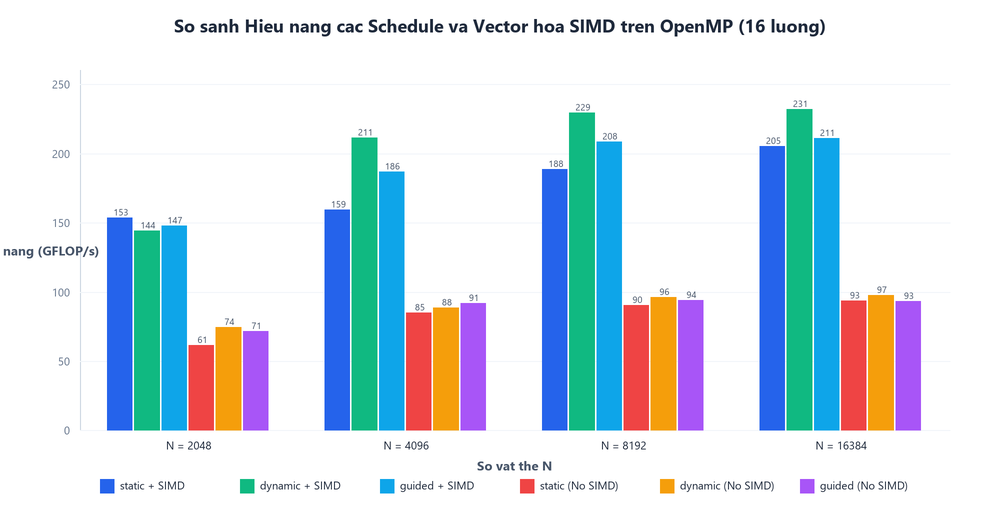
\includegraphics[width=\linewidth]{ntduong_schedule_simd}
\end{column}
\begin{column}{0.43\textwidth}
\begin{itemize}\small
\setlength{\itemsep}{6pt}
\item \textbf{SIMD} nhanh hơn $\approx$\alert{2.2×} (bản tắt dùng \code{no-tree-vectorize})
\item \textbf{\code{dynamic}} nhanh hơn \code{static} 13--33\%: lõi P làm xong thì lấy thêm việc
\item \textbf{Newton 3} ($N^2/2$ cặp) lại \alert{chậm hơn} 1.2--2.3×: ghi phân tán, mất SIMD, mảng đệm 4 MB
\end{itemize}
\end{column}
\end{columns}
\end{frame}

% =====================================================================
\section{CUDA}
\nguoinoi{Trình bày: Trần Tiến Đạt}

\begin{frame}{CUDA: kernel tiled dùng shared memory [1]}
\centering
\begin{tikzpicture}[>=Stealth, font=\small, scale=0.9, transform shape, box/.style={draw, minimum height=0.6cm, align=center}]
  \foreach \k/\t in {0/Tile 0, 1/Tile 1, 2/Tile 2, 3/$\cdots$, 4/Tile $k$} {
    \node[box, minimum width=1.8cm, fill=black!5] (g\k) at (\k*1.95,2.4) {\t};
  }
  \node[box, minimum width=1.8cm, fill=orange!30] at (g2) {Tile 2};
  \node[font=\scriptsize\itshape, anchor=east] at (-1.1,2.4) {global memory};
  \node[box, minimum width=3.6cm, fill=orange!30] (sh) at (3.9,1.2) {\code{shPos[0..B-1]}};
  \node[font=\scriptsize\itshape, anchor=east] at (-1.1,1.2) {shared memory};
  \draw[->, thick] (g2.south) -- (sh.north);
  \foreach \k/\t in {0/Luồng 0, 1/Luồng 1, 2/$\cdots$, 3/Luồng $B-1$} {
    \node[box, minimum width=1.8cm, fill=chinh!10] (t\k) at (\k*2.6,0) {\t};
    \draw[->] (sh.south) -- (t\k.north);
  }
  \node[font=\scriptsize\itshape, anchor=east] at (-1.1,0) {thanh ghi};
\end{tikzpicture}
\vspace{2pt}
\begin{itemize}\small
\setlength{\itemsep}{2pt}
\item 1 luồng = 1 vật thể. \textbf{Naive} đọc thẳng global memory: 20 FLOP / 16 byte $= 1.25$ FLOP/byte $\ll 25.3$ của T4 $\Rightarrow$ \alert{nghẽn bộ nhớ}
\item \textbf{Tiled}: cả khối nạp chung 1 tile rồi mỗi luồng dùng lại $B$ lần $\Rightarrow$ đọc global memory giảm $B$ lần
\item \code{\_\_syncthreads()} 2 lần: chờ nạp xong rồi mới đọc; chờ dùng xong rồi mới nạp tile mới
\end{itemize}
\end{frame}

\begin{frame}{CUDA trên Tesla T4: kết quả}
\begin{columns}[T]
\begin{column}{0.55\textwidth}
\centering
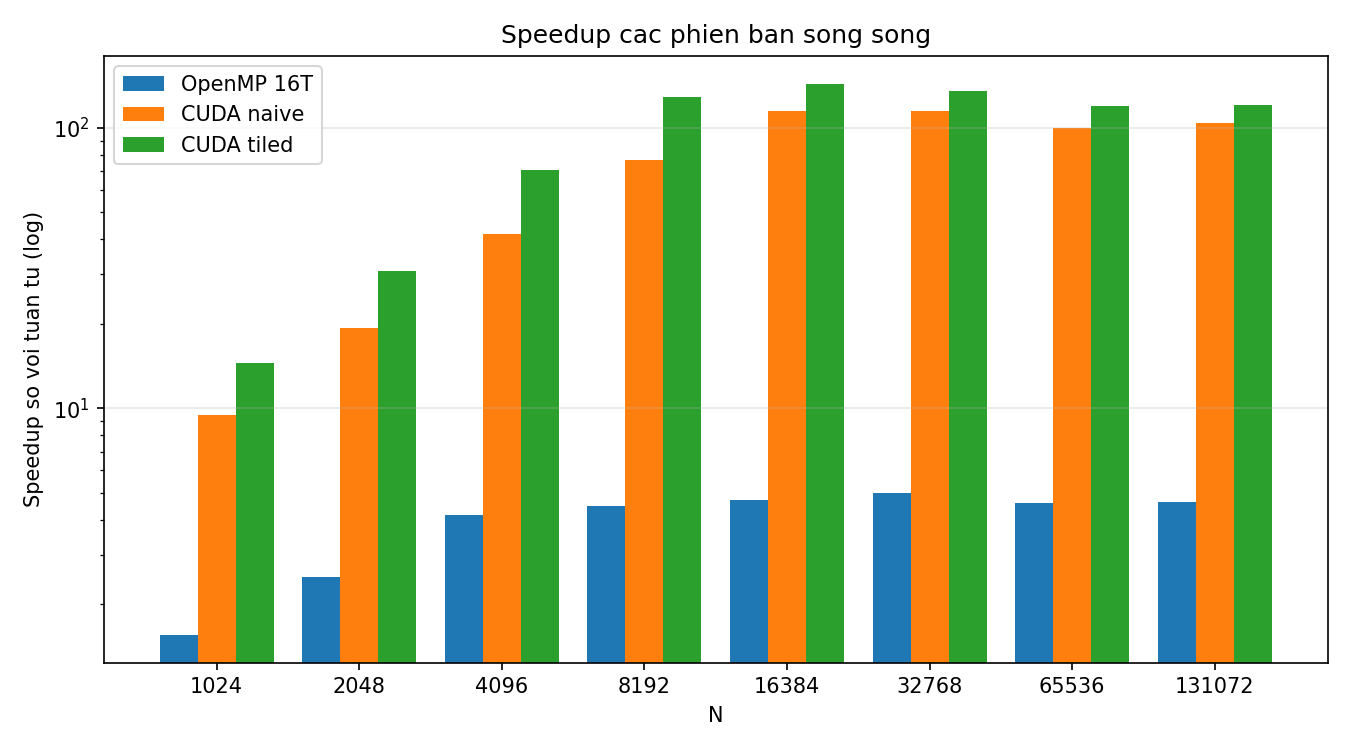
\includegraphics[width=\linewidth]{gpu_speedup}
\end{column}
\begin{column}{0.43\textwidth}
\centering
\so{4.7}{TFLOP/s, tiled, $N=16384$\\$\approx$ 58\% đỉnh FP32 của T4}
\vspace{6pt}
\begin{itemize}\small
\setlength{\itemsep}{3pt}
\item Tiled nhanh hơn naive 1.5--1.7× ($N\le8192$), còn $\approx$1.2× khi $N$ lớn (L1/L2 đỡ cho naive)
\item Kích thước khối 64--512 chênh $<4\%$, $B=256$ tốt nhất
\item Chép CPU$\leftrightarrow$GPU chỉ \alert{0.29\%} thời gian ở $N=131072$ (dữ liệu nằm trên GPU suốt mô phỏng)
\end{itemize}
\end{column}
\end{columns}
\end{frame}

% =====================================================================
\section{Kết luận}
\nguoinoi{Trình bày: Nguyễn Quốc Doanh}

\begin{frame}{So sánh tổng hợp: thời gian mỗi bước theo $N$}
\begin{columns}[T]
\begin{column}{0.55\textwidth}
\centering
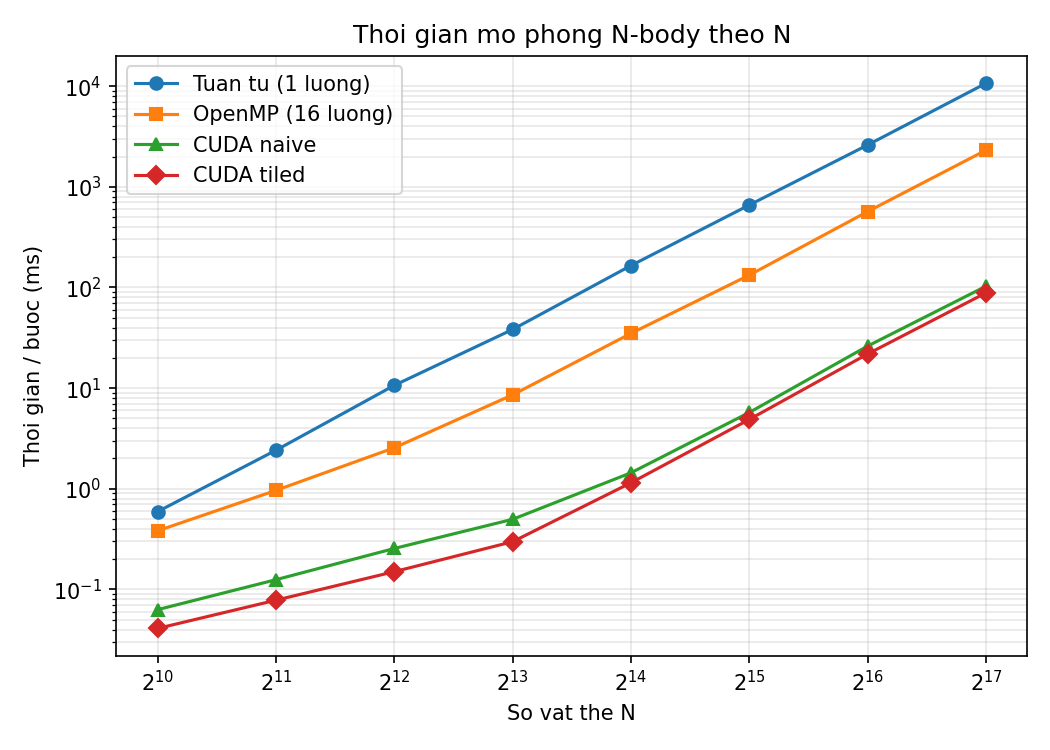
\includegraphics[width=\linewidth]{time_vs_n}
\end{column}
\begin{column}{0.43\textwidth}
\centering
\so{4.8×}{OpenMP so với tuần tự, $N=131072$}\\[10pt]
\so{132×}{CUDA tiled so với tuần tự (28× so với OpenMP)}
\vspace{6pt}
\begin{itemize}\scriptsize
\item Độ dốc $\approx2$ trên log--log: xác nhận $O(N^2)$
\item CPU, GPU đo trên 2 máy: so sánh bậc độ lớn
\end{itemize}
\end{column}
\end{columns}
\end{frame}

\begin{frame}{Kết luận và hướng phát triển}
\begin{itemize}
\setlength{\itemsep}{5pt}
\item Cả 4 phiên bản cho kết quả khớp nhau, năng lượng bảo toàn tốt
\item OpenMP 4.8--5.9× trên CPU lai; CUDA tiled 132×, 4.7 TFLOP/s
\item Kết quả khớp lý thuyết: speedup tăng theo $N$ (Gustafson); giới hạn thực tế đến từ phần cứng
\item \alert{Bài học: cách truy cập bộ nhớ quan trọng không kém số phép tính}\\
{\small Newton 3 tính ít hơn mà chậm hơn; tiled tính bằng naive mà nhanh hơn}
\end{itemize}
\vspace{4pt}
\textbf{Hướng phát triển:} Barnes--Hut $O(N\log N)$; nhiều GPU + MPI; tối ưu kernel (thread coarsening, CUDA streams)
\end{frame}

\nguoinoi{}
\begin{frame}[plain]
\centering\vfill
{\huge\bfseries\color{chinh} Cảm ơn thầy cô và các bạn đã lắng nghe}\\[16pt]
{\small Mã nguồn và số liệu: \code{github.com/doanh9a246-afk/motcongmotbangmay}}\\[20pt]
{\scriptsize\color{gray}
[1] L. Nyland, M. Harris, J. Prins, ``Fast N-Body Simulation with CUDA,'' \emph{GPU Gems 3}, Ch.~31, 2007.\\ \relax
[2] OpenMP Architecture Review Board, \emph{OpenMP API Specification} 5.2, 2021.}
\vfill
\end{frame}

\end{document}
